\documentclass[10pt]{article}
\usepackage[polish]{babel}
\usepackage[utf8]{inputenc}
\usepackage[T1]{fontenc}
\usepackage{graphicx}
\usepackage[export]{adjustbox}
\graphicspath{ {./images/} }
\usepackage{amsmath}
\usepackage{amsfonts}
\usepackage{amssymb}
\usepackage[version=4]{mhchem}
\usepackage{stmaryrd}

\title{Ak Akademia \\
 Pomorska \\
 w Stupsku }

\author{}
\date{}


\begin{document}
\maketitle
\begin{center}

\includegraphics[max width=\textwidth]{2024_11_21_6db36f485c30a3a4f8d0g-1}
\end{center}

\begin{center}
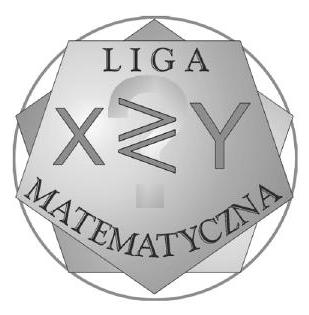
\includegraphics[max width=\textwidth]{2024_11_21_6db36f485c30a3a4f8d0g-1(1)}
\end{center}

\section*{LIGA MATEMATYCZNA \\
 im. Zdzisława Matuskiego \\
 PÓŁFINAŁ 15 marca 2022 \\
 SZKOŁA PODSTAWOWA \\
 klasy IV - VI}
\section*{ZADANIE 1.}
Zestaw \(A\) zawiera dziesięć różnych liczb jednocyfrowych. Adam wykreślił jedną liczbę, otrzymując zestaw \(B\). Suma wszystkich liczb w tym zestawie to 39. Spośród nich Adam wykreślił dwie liczby, uzyskując zestaw \(C\) o sumie liczb równej 37. Następnie usunął jeszcze trzy liczby, których suma jest równa 22 . Zestaw \(D\) składa się z liczb, które pozostały. Podaj największą liczbę zestawu \(D\).

\section*{ZADANIE 2.}
Flamastry w sklepie papierniczym zapakowane są w pudełka po 3 lub po 5 sztuk. Wszystkich pudełek jest 30, a w nich łącznie 110 flamastrów. Ile jest pudełek z trzema flamastrami?

\section*{ZADANIE 3.}
Jaki jest najmniejszy możliwy obwód trójkąta, którego każdy bok ma inną długość, a długość każdego boku jest liczbą pierwszą?

\section*{ZADANIE 4.}
Z cyfr 1,2,3,4,5,6,7,8,9 Basia wybrała cztery kolejne, z których ułożyła liczby czterocyfrowe podzielne przez 36. Ile było tych liczb?

\section*{ZADANIE 5.}
Z czterech jednakowych prostokątów i czterech jednakowych kwadratów Ania ułożyła kwadrat o obwodzie 32. Potem z tych samych czworokątów powstała figura przedstawiona na drugim rysunku. Oblicz obwód drugiej figury.\\
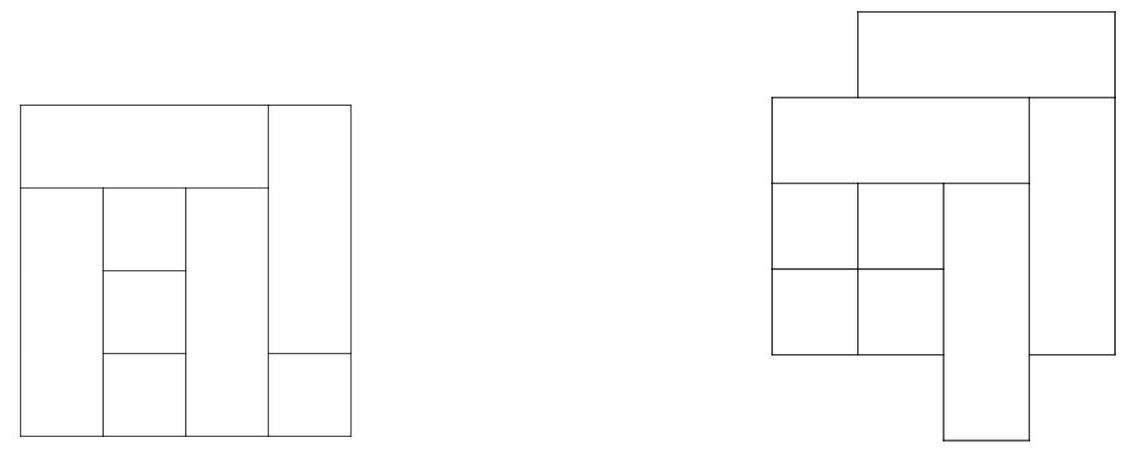
\includegraphics[max width=\textwidth, center]{2024_11_21_6db36f485c30a3a4f8d0g-1(2)}


\end{document}